% Type of the document
\documentclass[11pt]{beamer}

% elementary packages:
\usepackage{graphicx}
%\usepackage[latin1]{inputenc}
\usepackage[T1]{fontenc}
\usepackage[vietnamese]{babel}
%\usepackage[utf8]{vietnam} 
\usepackage{listings}
\usepackage{xcolor}
\usepackage{eso-pic}
\usepackage{mathrsfs}
\usepackage{url}
\usepackage{amssymb}
\usepackage{amsmath}
\usepackage{multirow}
\usepackage{hyperref}
\usepackage{booktabs}
\usepackage{tikz}
\usetikzlibrary{arrows.meta}
\usepackage{xcolor}
\usepackage{bm}
\newcommand*{\B}[1]{\ifmmode\bm{#1}\else\textbf{#1}\fi}



% additional packages
\usepackage{bbm}

% packages supplied with ise-beamer:
\usepackage{cooltooltips}
\usepackage{colordef}
\usepackage{beamerdefs}
\usepackage{lvblisting}

% Mathematics
\usepackage{amssymb}
\usepackage{amsmath}
\usepackage{mathrsfs}
\usepackage{amsthm,amsfonts}
\usepackage{mathtools}
\usepackage{algorithmic}
\usepackage[linesnumbered,ruled]{algorithm2e}
\usepackage{float}
\newcommand{\ra}{\rightarrow}
\newcommand{\Ra}{\Rightarrow}
\newcommand{\lra}{\longrightarrow}
\newcommand{\Lra}{\Longrightarrow}
\newcommand{\la}{\leftarrow}
\newcommand{\La}{\Leftarrow}
\newcommand{\lla}{\longleftarrow}
\newcommand{\Lla}{\Longleftarrow}
\newcommand{\Llra}{\Longleftrightarrow}
\newcommand{\map}{\longmapsto}
\newcommand{\al}{\alpha}
\newcommand{\bt}{\beta}
\newcommand{\dt}{\delta}
\newcommand{\De}{\Delta}
\newcommand{\tta}{\theta}
\newcommand{\e}{\varepsilon}
\newcommand{\vp}{\varphi}
\newcommand{\na}{\nabla}
\newcommand{\pa}{\partial}
\newcommand{\sm}{\sigma}
\newcommand{\Sm}{\Sigma}
\newcommand{\Gm}{\Gamma}
\newcommand{\gm}{\gamma}
\newcommand{\Om}{\Omega}
\newcommand{\R}{\mathbb R}
\newcommand{\Q}{\mathbb Q}
\newcommand{\N}{\mathbb N}
\newcommand{\Z}{\mathbb Z}
\newcommand{\Oo}{\mathcal O}
\newcommand{\K}{\mathcal K}
\newcommand{\G}{\mathcal G}
\newcommand{\D}{\mathcal D}
\newcommand{\X}{\mathcal X}
\newcommand{\M}{\mathcal M}
\newcommand{\T}{\mathcal T}
\newcommand{\V}{\mathcal V}
\newcommand{\W}{\mathcal W}
\newcommand{\PP}{\mathcal P}
\newcommand{\QQ}{\mathcal Q}
\newcommand{\UU}{\mathcal U}
\newcommand{\LL}{\mathcal L}
\newcommand{\cbe}{\scriptsize}
\newcommand{\On}{\widetilde{\mathcal{O}}}
\newcommand{\Mn}{\widetilde{M}}
\newcommand{\wt}[1]{\widetilde #1}
\newcommand{\sumh}{\overline{\sum}}
\newcommand{\cho}[2]{\ensuremath{#1\choose#2}}
\newcommand{\ve}[1]{{\bf #1}}

\DeclareMathOperator{\Div}{div}
\DeclareMathOperator{\Vol}{Vol}
\DeclareMathOperator*{\argmin}{argmin}
\DeclarePairedDelimiter{\norm}{\lVert}{\rVert}
\DeclarePairedDelimiter{\abs}{\lvert}{\rvert}

\newtheorem{Not}{Notation}
\newtheorem{Hypo}{Hypothesis}
\newtheorem{Theo}{Theorem}%[section]
\newtheorem{Prop}{Proposition}%[section]
\newtheorem{Coro}{Corollary}%[section]
\newtheorem{Algo}{Algorithm}

\theoremstyle{definition}
\newtheorem{Defi}{Definition}%[section]

\theoremstyle{plain}
\newtheorem{Lem}{Lemma}%[section]
\theoremstyle{plain}
\newtheorem{Assu}{Assumption}
\usepackage[backend=biber,style=numeric, citestyle=ieee]{biblatex}
\addbibresource{sample.bib}
\theoremstyle{remark}
\newtheorem*{Rem}{Remark}
%\usepackage{caption}
\usepackage{subcaption}


% Change the pictures here:
% logobig and logosmall are the internal names for the pictures: do not modify them. 
% Pictures must be supplied as JPEG, PNG or, to be preferred, PDF
\pgfdeclareimage[height=3cm]{logobig}{Figures/logoptit}
% Supply the correct logo for your class and change the file name to "logo". The logo will appear in the lower
% right corner:
\pgfdeclareimage[height=1cm]{logosmall}{Figures/logoptit}

% Title page outline:
% use this number to modify the scaling of the headline on title page
\renewcommand{\titlescale}{1.0}
% the title page has two columns, the following two values determine the percentage each one should get
\renewcommand{\titlescale}{1.0}
\renewcommand{\leftcol}{0.6}

% smaller font for selected slides
\newcommand\Fontvi{\fontsize{10}{7.2}\selectfont}
\newcommand\Fontsm{\fontsize{8}{7.2}\selectfont}
%\usepackage{caption}

% Define the title. Don't forget to insert an abbreviation instead 
% of "title for footer". It will appear in the lower left corner:
\title[ \footnotesize  \textcolor{red}{\bf Đồ án tốt nghiệp} -- \textcolor{blue}{Trần Xuân Độ }]{\Large  \bf ĐỒ ÁN TỐT NGHIỆP ĐẠI HỌC}


% Define the authors:
\authora{\bfseries \textcolor{blue}{\Large Chủ đề: Bao lồi và ứng dụng trong việc định hướng và phát hiện đối tượng có hướng}\vspace{20pt}} % a-c

\authorb{ Giảng viên hướng dẫn: Nguyễn Kiều Linh}
\authorc{Sinh viên thực hiện: Trần Xuân Độ - B19DCCN183 \\ 
	\hspace{3.6cm} Đặng Thị Thoa - B19DCCNxxx} 

% Define the institute:
\institute{\bf  Hà Nội, tháng 12 năm 2023}

% Comment the following command, if you don't want, that the pdf file starts in full screen mode:
\hypersetup{pdfpagemode=FullScreen}

%%%%
% Main document
%%%%
\setbeamertemplate{section in toc}[square]
\setbeamertemplate{subsection in toc}[ball unnumbered]
\AtBeginSection[]
{
	\begin{frame}
		\frametitle{Nội dung chính}
		\tableofcontents[currentsection]
	\end{frame}
}% mỗi đầu section thì thêm 1 frame mục lục làm nổi bật section đó%
\AtBeginSubsection[]
{
	\begin{frame} 
		\frametitle{Nội dung chính}
		\tableofcontents[currentsection,currentsubsection]
	\end{frame}
}

\begin{document}
%	\frame[plain]{%
%		\titlepage{}
%	}

	\section{Giới thiệu bài toán}
	\subsection{Đặt vấn đề}
	\begin{frame}{Đặt vấn đề}
			Thách thức lớn: đặc trưng răng cưa (feature aliasing)
			\begin{columns}[c] % Căn giữa các cột
			\column{.5\textwidth} % Cột 1 chiếm 50% của khung
			\begin{figure}
				\centering
				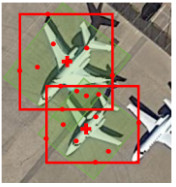
\includegraphics[width=3cm]{reppoint_bouding_box.jpg}
		
			\end{figure}
			\column{.5\textwidth} % Cột 2 chiếm 50% của khung
			\begin{figure}
				\centering
				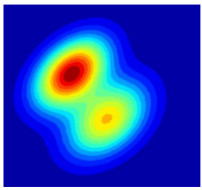
\includegraphics[width=3cm]{reception_field_w_aliasing.jpg}
			
			\end{figure}
		\end{columns}
	\end{frame}
	
	
	\begin{frame} {Giải quyết vấn đề}
		Sử dụng bao lồi làm biểu diễn bounding box.
		\begin{columns}[c] % Căn giữa các cột
			\column{.5\textwidth} % Cột 1 chiếm 50% của khung
			\begin{figure}
				\centering
				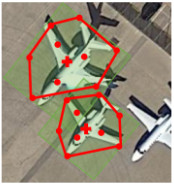
\includegraphics[width=3cm]{ConvexHull_Bouding_Box.jpg}
			
			\end{figure}
			
			\column{.5\textwidth} % Cột 2 chiếm 50% của khung
			\begin{figure}
				\centering
				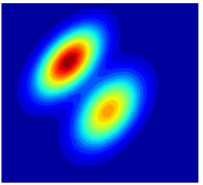
\includegraphics[width=3cm]{reception_field_wo_aliasing.jpg}
			
			\end{figure}
		\end{columns}
	\end{frame}
	\subsection{Phương pháp thích ứng bao lồi (convex-hull feature adaptation-CFA)}
	
	\begin{frame}{Phương pháp thích ứng bao lồi (convex-hull feature adaptation-CFA)}
	 
	 Giới hạn phạm vi đối tượng sử dụng chỉ số CIoU.\\
	 Phân chia tập bao lồi thành bao lồi âm và bao lồi dương.
		\begin{figure}[htp]
			\begin{center}
				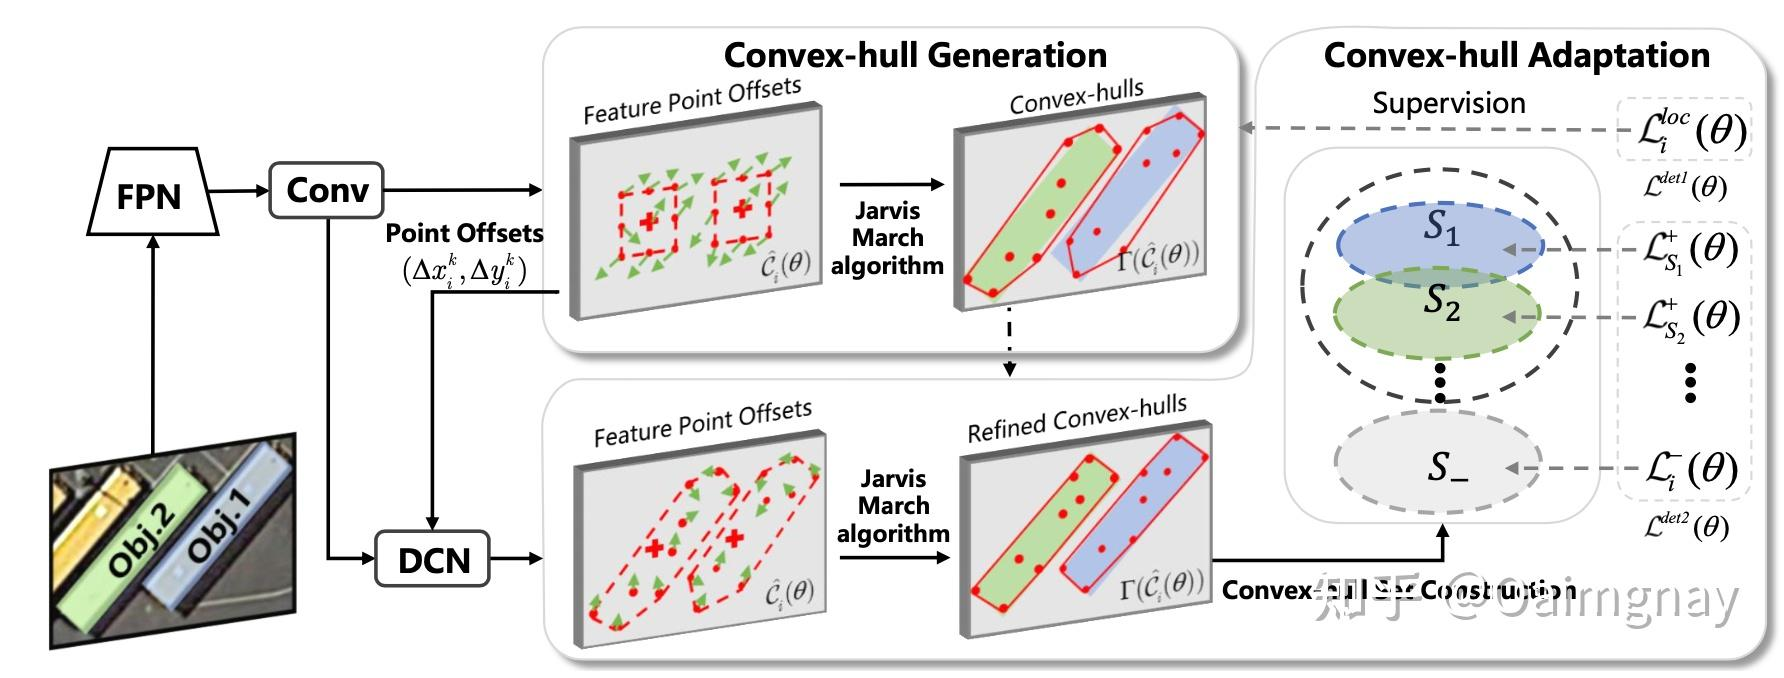
\includegraphics[width=10cm]{./Hinh_1.jpg}
			\end{center}
		\end{figure}
	\end{frame}
	\begin{frame}{Xây dựng tập bao lồi}
		
		Phương pháp CFA đã đề xuất biểu diễn phạm
		vi của đối tượng bằng bao lồi:\\
		\begin{align} \label{ptdd}
			C_i = \{(x_i^k, y_i^k )\}_i^{k=1,2,...,K}
		\end{align}
		
	
		
	\end{frame}
	\begin{frame}{2 giai đoạn thực hiện:}
		\begin{itemize}
			\item[I.] Tạo và ước lượng bố cục bao lồi.
			
			\item[II.] Chỉnh sửa bao lồi để phù hợp với các đối tượng dày đặc.
			
		\end{itemize}	
	\end{frame}
	
	
\begin{frame}{Giai đoạn I}
	Dự đoán độ lệch:
	\begin{align} \label{ptdd}
		\widehat C_l (\theta) \gets \{(x_i^k + \Delta x_i^k, y_i^k + \Delta y_i^k )\}_i^{k=1,2,...,K}
	\end{align}
\begin{figure}[ht!]
	\begin{center}
		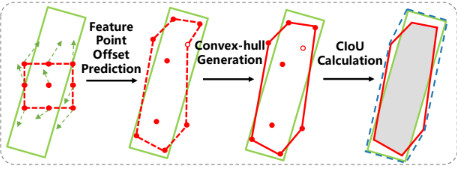
\includegraphics[width=8cm]{./feature_point_offset_prediction.jpg}
	\end{center}
\end{figure}
\end{frame}
	
	\begin{frame}{Tích chập biến dạng}
		Hỗ trợ lấy mẫu ở những vị trí đa dạng hơn => làm giàu dữ liệu.
		
		\begin{figure}[ht!]
			\begin{center}
				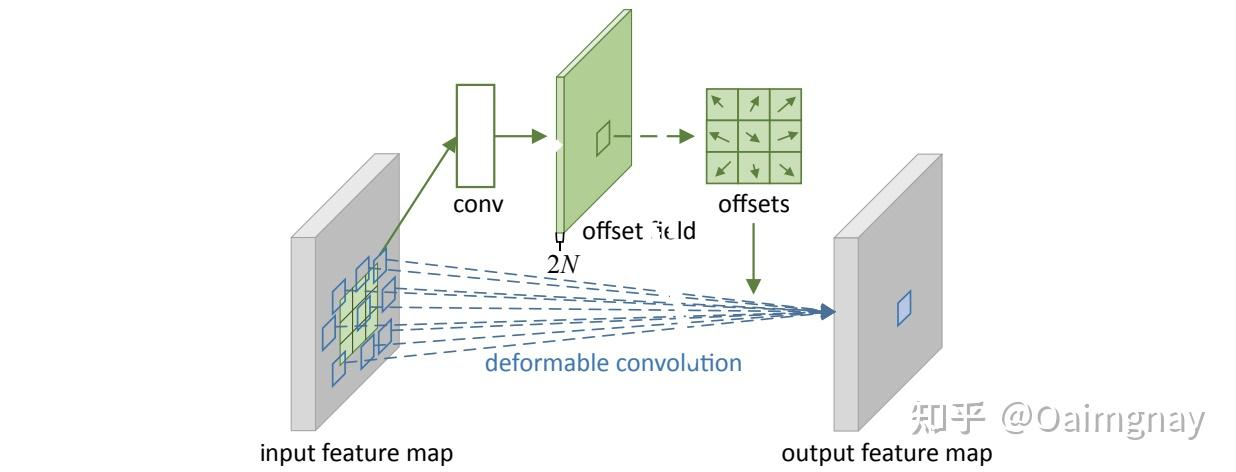
\includegraphics[width=8cm]{./Hinh_6.jpg}
			\end{center}
		\end{figure}
		
	\end{frame}
	
	
	\begin{frame}{Thuật toán tìm bao lồi}
	
		\begin{itemize}
			\item[-] Thuật toán tìm bao lồi xấp xỉ -  Convex Approximation.
			\item[-]  Thuật toán tìm bao lồi trực giao - Orthogonal Quick Hull.
			
			Tìm một bao lồi tối thiểu cho 9 điểm feature point offset.
			
		\end{itemize}
	\end{frame}
	
	\begin{frame}{Định nghĩa công thức Convex Intersection over Union (CIoU)}
		\begin{figure}[ht!]
			\begin{center}
				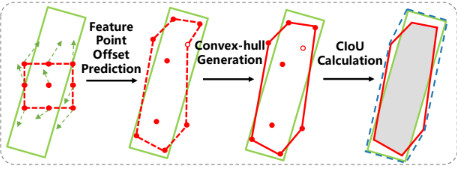
\includegraphics[width=8cm]{./feature_point_offset_prediction.jpg}
			\end{center}
		\end{figure}
		\begin{align} 
			CIoU_{(C_i (\theta), B_j)} (\theta) = \frac{|C_i(\theta) \cap B_j|}{|C_i(\theta) \cup B_j|} - \frac{|R_j \setminus (C_i(\theta) \cup B_j)|}{|R_j|}
		\end{align}
	\end{frame}
	
	
	\begin{frame}{Convex-Hull Localization Loss}
		\begin{align} \label{ptdd0}
			\mathcal{L}_i^{loc} (\theta) = 1 - CIoU(C_i(\theta), B_j)
		\end{align}
		
	\end{frame}
	\begin{frame}{Convex-hull Classification Loss}
	
		\begin{align} \label{ptdd1}
			\mathcal{L}	_i^{cls} (\theta) =FL(S_i(\theta), Y_j) 
		\end{align}
	
	\end{frame}
	\begin{frame}{Convex-hull Loss}
		Hàm loss phân loại cho bao lồi dương:\\
		\begin{align} \label{ptdd2}
			\mathcal{L}^+ (\theta) = 	\mathcal{L}_i^{cls}(S_i(\theta), Y_j) +\lambda 	\mathcal{L}_i^{loc}(C_i(\theta), B_j)
		\end{align}
		Hàm loss phân loại cho bao lồi âm:\\
		\begin{align} \label{ptdd3}
			\mathcal{L}^- (\theta) = \mathcal{L}_i^{cls}(S_i(\theta), Y_j) 
		\end{align}
		
	\end{frame}
	\begin{frame}{Tối ưu quá trình huấn luyện}
		\begin{equation}
			\mathcal{L}^{\text {det } 1}(\theta)=\frac{1}{J} \sum_i \mathbb{I}_{\left(x_i, y_i\right)} \mathcal{L}_i^{l o c}(\theta)
		\end{equation}
	\end{frame}
	\begin{frame}{Thích ứng bao lồi - Convex Hull Adaptation}
		Xử lý hiện tượng feature aliasing. \\
		\textbf{Convex-Hull Set Construction}: Xây dựng một tập các bao lồi cho mỗi đối tượng.
		\begin{figure}[ht!]
			\begin{center}
				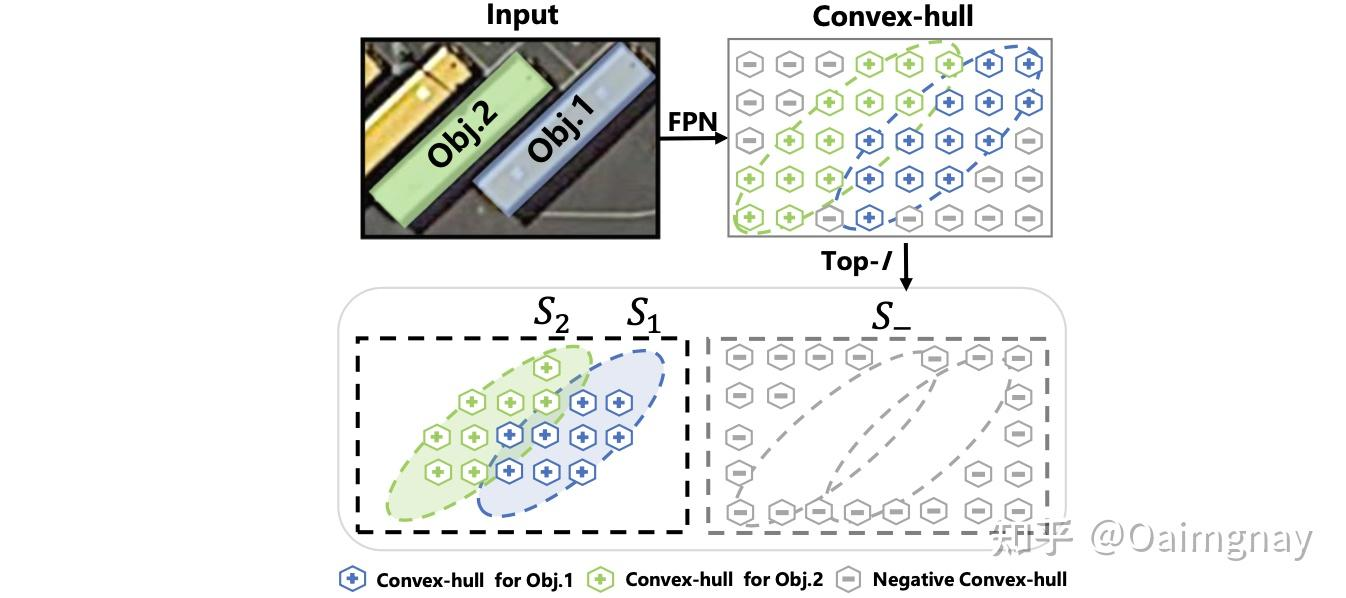
\includegraphics[width=10cm]{./Hinh_8.jpg}
			\end{center}
		\end{figure}
	\end{frame}
	
	\begin{frame}{Xây dựng tập các bao lồi}
		Tập các bao lồi dương($S_j$) được xây dựng bằng cách chọn ra $\text{top-I}$ bao lồi làm bao lồi dương, theo CIoU giữa các bao lồi và các hộp thật của đối tượng (grouth-truth).\\
		Các bao lồi khác mà không thuộc đối tượng nào sẽ được gộp vào tập các bao lồi âm ($S_{\_}$).
	\end{frame}
	
	
	
	\begin{frame}{Chiến lược chia tập các bao lồi}
		Cách chia tập các bao lồi được hướng dẫn bởi nguyên tắc nhất quán đạo hàm. Lấy đạo hàm của phương trình(\ref{pt11}), có đạo hàm của tập các bao lồi:
		\begin{align} \label{ptdd7}
			\frac{\partial\mathcal{L}_{S_j}^+ (\theta)}{\partial (\theta)} = \frac{1}{|S_j|} \sum_{i \in {S_j}} \frac{\partial (f(\mathcal{L}_i^+(\theta))\mathcal{L}_i^{+}(\theta))}{\partial (\mathcal{L}_i^+(\theta))} \frac{\partial \mathcal{L}_i^+ (\theta)}{\partial (\theta)}
		\end{align}
		
	\end{frame}
	

	
	\begin{frame}{Chiến lược phân đoạn tập các bao lồi}
		
		\begin{figure}[ht!]
			\begin{center}
				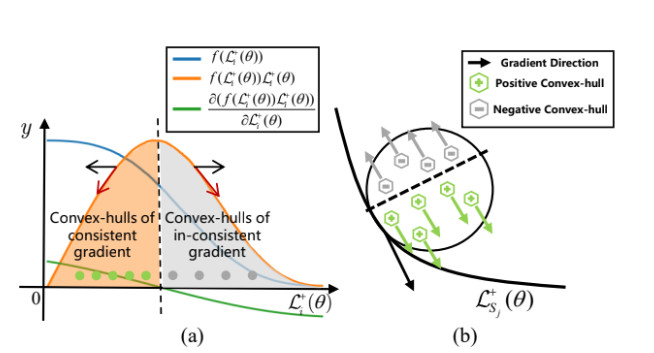
\includegraphics[width=10cm]{./Hinh_9.jpg}
				\caption{Chia tách tập convex-hull dựa trên nguyên tắc tính thống nhất gradient.}
				\label{upper_convex_function}
			\end{center}
		\end{figure}
		
	\end{frame}
	\begin{frame}{Xử lý hiện tượng đặc trưng răng cưa}
		Đưa ra công thức tính hệ số khử đặc trưng răng cưa:
		\begin{align} \label{ptdd8}
			p_i = \gamma \frac{CIoU (\mathcal{C}_i, \mathcal{B}_j)}{\sum_{m=1}^{M} CIoU (\mathcal{C}_i, \mathcal{B}_m)}
		\end{align}
	
		
		
	\end{frame}
	\begin{frame}{Tối ưu hàm loss giai đoạn 2}
		Việc tối ưu của giai đoạn 2 được điều khiển bởi sự kết hợp cả hàm loss classification và localization định nghĩa trên tập các bao lồi:\\
		\begin{align} \label{ptdd10}
			\mathcal{L}^{det2} (\theta) = \frac{1}{J} \sum_{j=1}^{J} \frac{1}{|S_j|} \sum_{i \in {S_j}} p_i f(\mathcal{L}_i^+(\theta)) \mathcal{L}_i^{+}(\theta)  + \frac{1}{|S_-|} \sum_{i \in S} \mathcal{L}_i^- (\theta) 
		\end{align}
	\end{frame}
	\begin{frame}{Hàm loss của bộ phát hiện CFA}
		Là tổng hàm loss của cả hai giai đoạn:
		\begin{align}
			\mathcal{L}_{CFA} = \mathcal{L}^{\operatorname{det} 1}(\theta)+\mathcal{L}^{\operatorname{det} 2}(\theta)
		\end{align}
		
	\end{frame}
	
	
	\section{Thuật toán tính bao lồi xấp xỉ}
	\subsection{Outer convex approximation}
	\begin{frame}{Thuật toán 1}
		Cho tập hợp các điểm trong không gian:
			\begin{figure}
		\begin{center}
			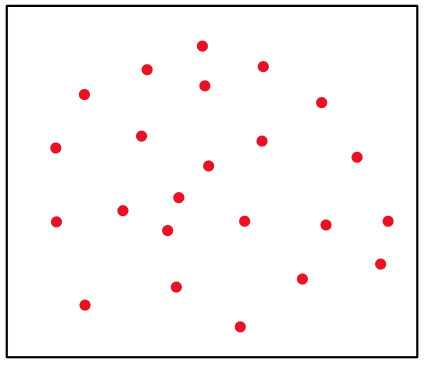
\includegraphics[width=6cm]{./initial_sub_point.jpg}
		\end{center}
	\end{figure}
	Cần tìm ra tứ giác bao quanh xấp xỉ các điểm này.
	\end{frame}
	\begin{frame}{Bắt đầu thuật toán}
		Khởi tạo hình chữ nhật lớn nhất bao quanh các điểm.
		\begin{figure}
		
			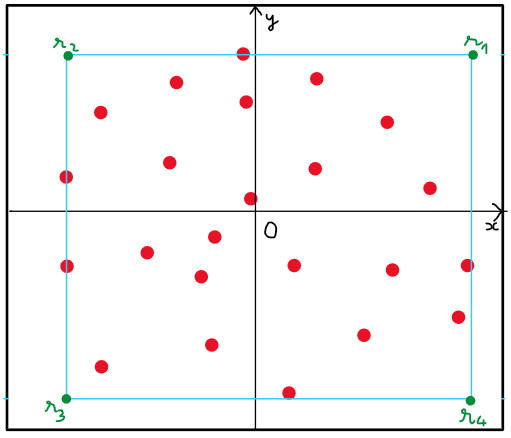
\includegraphics[width=6cm]{khoi_tao_hcn_bao_quanh}
		\end{figure}
	\end{frame}
	\begin{frame}
		Hình chữ nhật $\mathcal{P}^{outer}$ cấu tạo gồm 4 đỉnh như sau:
		Tập P ban đầu chứa 4 đỉnh này:\\
		\begin{equation}\label{def_4r-2}
			P := \{r_1,\ r_2,\ r_3,\ r_4\}
		\end{equation}
	\end{frame}
	\begin{frame}
		Lấy 1 đỉnh $p \in P$, có được $p^{-}$ là điểm liền trước (ngược chiều kim đồng hồ) của $p$, $p^{+}$ là điểm liền sau của $p$, ta tính được hướng $d_p$ của $p$ và ngưỡng $\beta_{dp}$:\\
		\begin{equation}\label{def_d_p}
			\begin{array}{lcl}
				d_{p}^T &:=& \|p^+ - p^-\|^{-1}\, R \, (p^+ - p^-)^T, \\
				\beta_{d_{p}} &:=& \max\{d_{p}\, x^T \mid x \in X\},
			\end{array}
		\end{equation}
		trong đó: 
		\begin{equation}\label{rotationmatrix}
			R := \begin{pmatrix}
				0 & 1 \\
				-1 & 0
			\end{pmatrix}
		\end{equation}
	\end{frame}
	\begin{frame}
		Vì R là ma trân xoay, thay vào công thức ngưỡng $d_p$ bên trên:
		\begin{equation}\label{def_d_p1}
			\|d_{p}\| = \|p^+ - p^-\|^{-1}\, \|(p^+ - p^-) R^T\| = \|p^+ - p^-\|^{-1}\, \|p^+ - p^-\| = 1.
		\end{equation}
	\end{frame}
	
	
	\begin{frame}
		Xét biểu thức định nghĩa $\mathcal{P}^{outer}$:
		\begin{equation}\label{pt15}
			d_p\, x^T \leq \beta_{d_p}.
		\end{equation}
		Trường hợp 1, nếu:
		\begin{equation}
			\label{betaequal}
			\beta_{d_p} = d_p\, p^+
		\end{equation}
		Thì ràng buộc (\ref{pt15}) sẽ không tạo đỉnh mới mà tạo thêm cạnh mới $[p^-, p^+]$ của $\mathcal{P}^{outer}$.\\
		Cho $d_{[p^-, p]}$ và $d_{[p, p^+]}$ là hai hướng cực đại từ $D$ định nghĩa hai cạnh $[p^-, p]$ và $[p, p^+]$ của đa giác $\mathcal{P}^{outer}$. Tuy nhiên hai cạnh này mặc định có sẵn => hai hướng trên trở nên thừa thãi. 
		
	\end{frame}
	
	\begin{frame}
		Chính vì thế nên khi thêm $d_p$ vào tập $D$ ta cần loại bỏ hai hướng $d_{[p^-, p]}$ và $d_{[p, p^+]}$ khỏi tập $D$ và đỉnh $p$ từ $P$:
		\begin{equation}\label{newDP2}
			\begin{array}{lcl}
				D &:=& (D \cup \{d_{p}\})\setminus \{d_{[p^-,p]}, d_{[p,p^+]}\}, \\
				P &:=& P \setminus \{p\}.
			\end{array}
		\end{equation}
	\end{frame}
	
	\begin{frame}
		Xét trường hợp 2, nếu:
		\begin{equation}\label{betagreater}
			\beta_{d_p} > d_p\, p^+
		\end{equation}
		và:
		\begin{equation}\label{greaterdelta}
			d_{p}\, p^T - \beta_{d_{p}} > \delta
		\end{equation}
		thì ràng buộc (\ref{pt15}) tạo thêm 2 đỉnh mới cho đa giác là $\hat p^-$ và $\hat p^+$ và được tính toán bởi:
		\begin{equation}\label{def_hatp}
			\begin{array}{lcl}
				\lambda_p &:=& (\beta_{d_p} - d_p\, p^{-T})/(d_p\, p^T - d_p\, p^{-T}) \in (0, 1), \\
				\hat p^- &:=& (1 - \lambda_p)\, p^{-T} + \lambda_p\, p^T, \\
				\hat p^+ &:=& (1 - \lambda_p)\, p^{+T} + \lambda_p\, p^T.
			\end{array}
		\end{equation}
	\end{frame}
	
	\begin{frame}
		Tiếp theo ta thêm $d_p$ vào $D$ và thay thế $p \in P$ bởi $\hat p^+$ và $\hat p^+$:
		\begin{equation}\label{newDP1}
			\begin{array}{lcl}
				D &:=& D \cup \{d_{p}\}, \\
				P &:=&(P \setminus \{p\}) \cup \{\hat p^-, \hat p^+\}.
			\end{array}
		\end{equation}
		Lặp lại các bước tương tự, ta sẽ tìm được một bao lồi xấp xỉ của tập hợp các điểm.
	\end{frame}
	
	\begin{frame}{Một vài kết quả của Outer Convex Approximation}
		\begin{figure}
			\begin{center}
				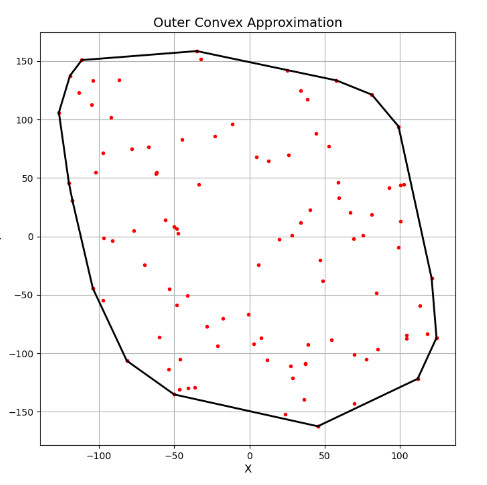
\includegraphics[width=6cm]{./result_outer_cv_delta0.jpg}
				\caption{Với n = 100, delta = 0.}
				\label{result_outer_cv_delta0}
			\end{center}
		\end{figure}
		
	\end{frame}
	\begin{frame}{Một vài kết quả của Outer Convex Approximation}
		\begin{figure}
			\begin{center}
				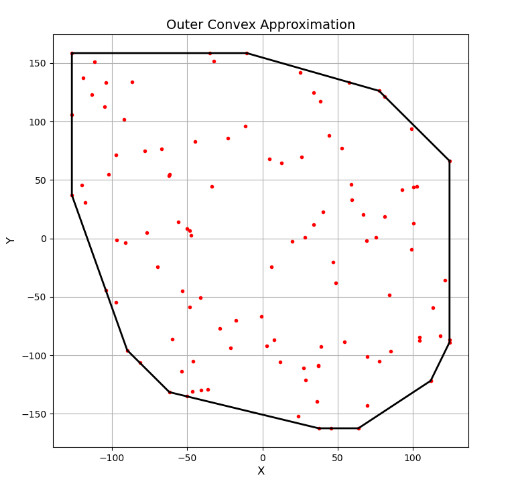
\includegraphics[width=6cm]{./result_outer_cv_delta20.jpg}
				\caption{Với n = 100, delta = 20.}
				\label{result_outer_cv_delta20}
			\end{center}
		\end{figure}
		
	\end{frame}
	\begin{frame}{Một vài kết quả của Outer Convex Approximation}
		\begin{figure}
			\begin{center}
				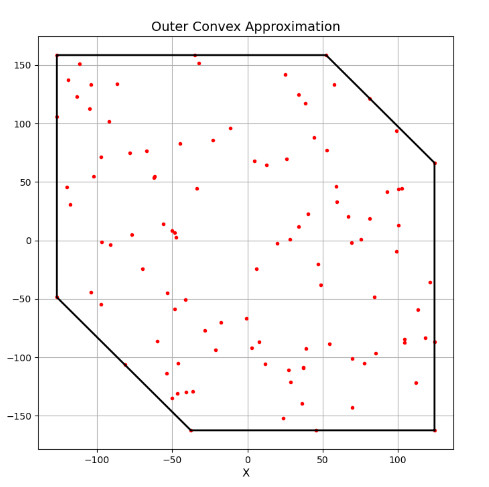
\includegraphics[width=6cm]{./result_outer_cv_delta50.jpg}
				\caption{Với n = 100, delta = 50.}
				\label{result_outer_cv_delta50}
			\end{center}
		\end{figure}
		s
	\end{frame}
	\section{Thuật toán tính bao lồi trực giao}
	\subsection{Các khái niệm liên quan}
	\begin{frame}{Bao lồi trực giao liên thông}
		
	\end{frame}
	\begin{frame}{Tính chất của bao lồi trực giao liên thông}
		
	\end{frame}
	\begin{frame}{Đường trực giao bên phải}
		
	\end{frame}
	
	\subsection{Thuật toán tìm bao lồi - Quickhull}
	\begin{frame}{ Thuật toán Quickhull}
		
	\end{frame}
	\begin{frame}{Tính đúng đắn và phức tạp của Quickhull}
		
	\end{frame}
	\section{Thực nghiệm và kết quả}
	\subsection{Môi trường}
	\begin{frame}{Thay thế bằng thuật toán Outer Convex Approximation}
		\textbf{Thay cả 2 hàm Jarvis() và Jarvis\_and\_index(), sử dụng full dataset}
	\end{frame}
	
\end{document}
